%\documentstyle[11pt,a4]{article}
%\documentclass[a4paper]{article}
\documentclass[12pt, a4paper]{article}
%\documentclass[a4paper, 10pt]{article}
% Seems like it does not support 9pt and less. Anyways I should stick to 10pt.
%\documentclass[a4paper, 9pt]{article}
\topmargin-2.0cm

%\usepackage{graphicx}
%\usepackage[english]{babel}
%\usepackage{fancyhdr}
%\usepackage{pagecounting}
%\usepackage[dvips]{color}

\usepackage{fancyhdr}
\usepackage{pagecounting}
\usepackage{cite}
\usepackage{comment}
\usepackage[dvipsnames]{xcolor}
\usepackage[compact]{titlesec}
\usepackage{graphicx}
\usepackage[skip=1pt]{caption}


% Color Information from - http://www-h.eng.cam.ac.uk/help/tpl/textprocessing/latex_advanced/node13.html

% NEW COMMAND
% marginsize{left}{right}{top}{bottom}:
%\marginsize{3cm}{2cm}{1cm}{1cm}
%\marginsize{0.85in}{0.85in}{0.625in}{0.625in}

\advance\oddsidemargin-0.65in
%\advance\evensidemargin-1.5cm
\textheight9.2in
\textwidth6.75in
\newcommand\bb[1]{\mbox{\em #1}}
\def\baselinestretch{1.05}
%\pagestyle{empty}

\newcommand{\hsp}{\hspace*{\parindent}}
\definecolor{gray}{rgb}{0.4,0.4,0.4}
%\definecolor{gray}{rgb}{1.0,1.0,1.0}


\begin{document}
\thispagestyle{fancy}
%\pagenumbering{gobble}
%\fancyhead[location]{text} 
% Leave Left and Right Header empty.
\lhead{}
\rhead{}
%\rhead{\thepage}
\renewcommand{\headrulewidth}{0.4pt} 
\renewcommand{\footrulewidth}{0.0pt} 

%\fancyfoot[C]{\footnotesize \textcolor{gray}{http://www.stanford.edu/$\sim$sundaes/application}}
\fancyfoot[C]{\textcolor{gray}{\thepage}} 

%\pagestyle{myheadings}
%\markboth{Sundar Iyer}{Sundar Iyer}

\pagestyle{fancy}
\lhead{\textcolor{gray}{\it Matthew Fisher}}
%\rhead{\textcolor{gray}{\thepage/\totalpages{}}}
%\rhead{\thepage}
%\renewcommand{\headrulewidth}{0pt} 
%\renewcommand{\footrulewidth}{0pt} 
%\fancyfoot[C]{\footnotesize http://www.stanford.edu/$\sim$sundaes/application} 
%\ref{TotPages}

\begin{small}

%\vspace*{0.1cm}
\begin{center}
{\LARGE \bf RESEARCH STATEMENT}\\
\vspace*{0.1cm}
{\normalsize Matthew Fisher (mdfisher@cs.stanford.edu)}\\
\vspace*{0.25cm}
{\large\textit{Creative Knowledge: Learning and Applying Example-Driven Representations}}
\end{center}
%\vspace*{0.2cm}

%\begin{document}
%\centerline {\Large \bf Research Statement for Sundar Iyer}
%\vspace{0.5cm}

% Write about research interests...
%\footnotemark
%\footnotetext{Check This}

My research focuses on seeking new representations for data with two objectives: (1) the representation should be directly applicable to some creative or labor-intensive task and (2) the representation should be trainable from observations, allowing it to both scale with the increasing availability of data and specialize to different needs. I am a strong believer that the trend away from hand-coded representations and towards data-driven methods will only continue, as even core staples of the community like the SIFT descriptor are facing strong competition from example-driven alternatives. This trend is driven in part by the proliferation of databases such as ImageNet and Flickr, but also by the new types of sensors and annotations that allow entirely new types of databases to be built and applied towards novel problems. One area that I focus on are commodity 3D sensors, such as the Microsoft Kinect and upcoming Google Tango, which have driven significant interest in using sensing technology for mapping and understanding the world. The proliferation of data made available by these sensors enables deep avenues of research that we have only begun to explore: 3D perception is vital to accurately understanding the identity and functionality of objects and the activities people perform in environments.

I believe that the representations used to make progress in both creative and physical modeling tasks will be championed by data-driven approaches that learn by observations of these events. This work rests at the intersection of graphics, machine learning, and vision, and my goal is to bring powerful tools from these fields together to create systems that have real impact on the world including content creation, robotics, virtual reality, and more. As the central pillar of the content creation stack in a wide range of fields, Adobe is in a unique position to push these research directions. I believe that Adobe, with access to a vast collection of expert-created content, is the ideal place for me to undertake this.

%\vspace{0.5cm}
\subsection*{Representing Creative and Natural Content}

\begin{figure}[b!!]
  \centering
    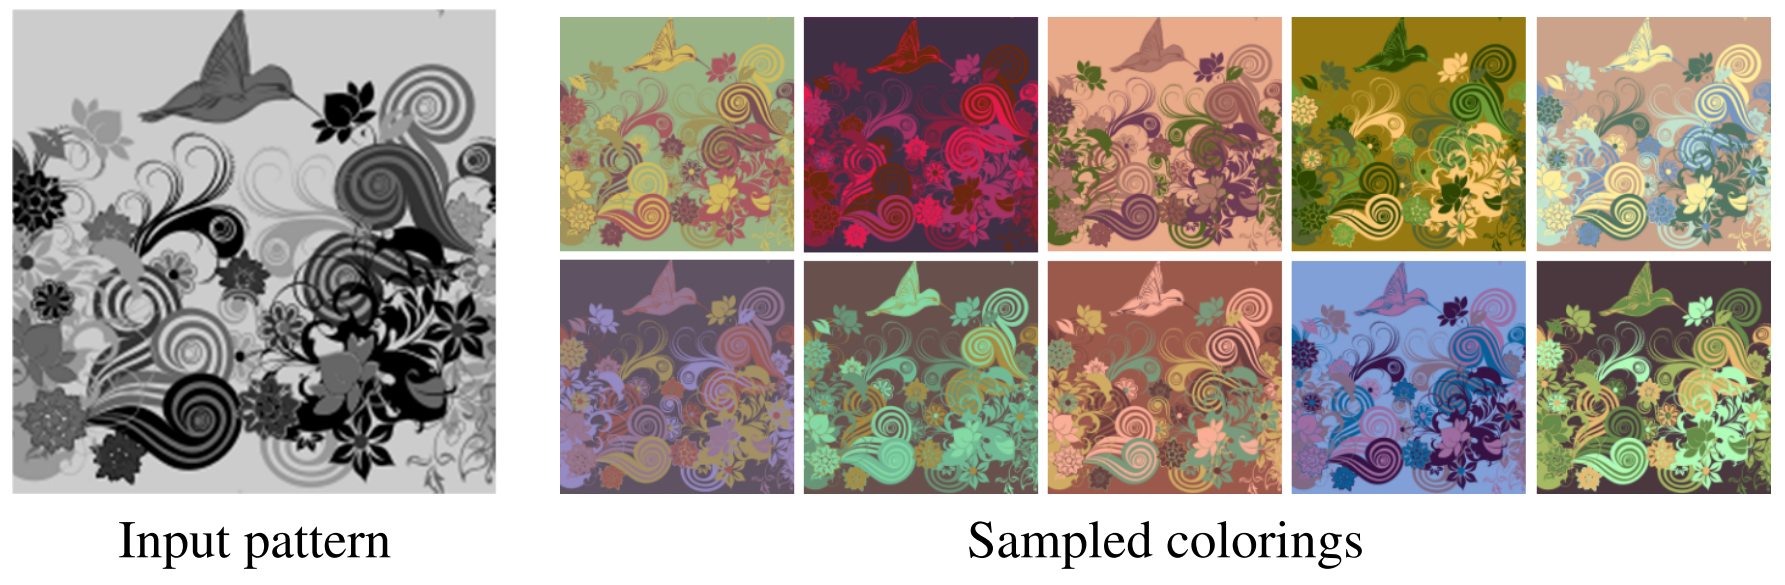
\includegraphics[width=\textwidth]{figColorSampling.png}
  \caption{\textit{Color-by-Numbers} trains a factor graph studies an artist's work and samples from this model to recolor images in their style.}
  \label{fig:colorSampling}  
\end{figure}

All creative tasks have an implied distribution over the space of content that the author seeks to sample from. Perhaps the goal is ``a cool-looking dinosaur'' subject to ``pretty and vibrant colors''. This distribution is impossible to accurately quantify, but like NP-complete problems, while generation is difficult it takes only a brief moment for the author to judge the acceptability of a candidate artifact. Motivated by this idea, I work to build systems that study collections of target content and  approximate the underlying distribution, then sample from it to generate a stream of content that can be further refined and modified. Numerous areas of graphics research can be cast in this light, ranging from texture synthesis to photograph retouching.

\paragraph{Coloring} Approaches to example-driven design differ wildly based on the type of content being modeled. In \emph{Color-by-Numbers}~\cite{colorByNumbers}, we used a factor graph to represent the distribution of different ways an artist might color an image, trying to capture both specific styles and abstract moods like ``pastel'', ``bold'', and ``mellow''. Although the representation itself was designed based on artistic principles like contrast and saliency, its parameters were driven entirely by samples drawn from the target distribution. Figure~\ref{fig:colorSampling} shows results sampled from this approach, enabling a vast collection of quality results to be generated almost instantly.

\paragraph{3D Modeling} In a system I designed for learning to synthesize 3D object arrangements from examples the representation was quite different: instead of a factor graph, a Bayesian network with a Gaussian mixture model captured the distribution of environments~\cite{exampleSynthesis}. The key insight that enabled this approach was to condition the representation on multiple sources of data: a broad corpus (in this case, a large indoor room collection) and a specialized set of exemplars. The broad corpus admits general knowledge, such as the expected distance and relative orientations between a bed and a nightstand, while the much smaller set of specialized exemplars helps the artist directly guide the synthesis towards sampling from the desired area. Figure~\ref{fig:exampleSynth} shows how this system supports synthesis with a tiny number of examples but produces scenes that draws diversity in both content and arrangements from the broader corpus.

\begin{figure}[h]
  \centering
    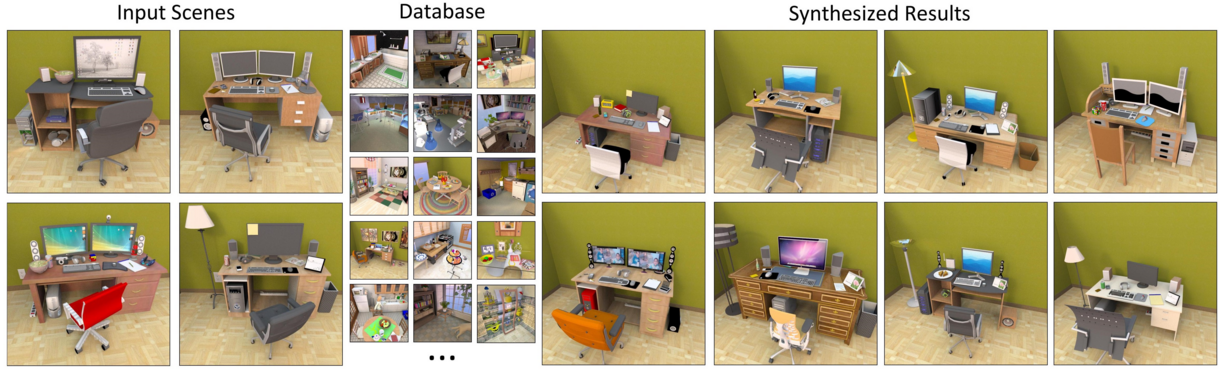
\includegraphics[width=\textwidth]{figExampleSynthesis.png}
  \caption{Example-based synthesis learns a distribution over object arrangements, incorporating both general knowledge from a large scene corpus and specific intent from targeted exemplars.}
  \label{fig:exampleSynth}  
\end{figure}

\paragraph{Generative Networks} Although different types of models have been employed in example-driven distributions including factor graphs, mixture models, and specialized algorithms like PatchMatch, the recent focus across many fields on deep learning approaches has strongly affected this avenue of research. The problem of learning generative representations of content is perfectly situated for deep networks and implementations can take advantage of the extensively optimized deep learning pipelines to process the growing quantities of available visual data. Many staples of generative design such as texture synthesis have been re-imagined with stellar results that far surpass every prior result, helping push these methods out of quaint novelties into usable technology. I believe this unification of approaches is only in its earliest stages, and am eager to help push this research frontier. Furthermore, Adobe is in an optimal position to not only feed these networks with the needed data, but to one day deploy these generative tools outside of academic settings into production environments.

\subsection*{Capturing and Processing the World at Scale}

Cameras capable of estimating depth alongside color are progressively more affordable and pervasive, and I focus on ways to both parse that raw data into a representation of the 3D world as well as analyze the captured environments to gain some understanding of the semantics of the environment. I believe this understanding is a key step towards helping machines interact beneficially with people in the real world. 

\paragraph{3D Scene Understanding} Great progress has been made on labeling objects by combining both 2D and 3D observations. But knowing an object's label is only the first step: vital questions like ``how can Mario interact with this living room?'' or ``how can the robot assist Hermione in cooking the eggs?'' require understanding not just the identity but also the functionality and usability of the objects in the environment. Following a generative approach to content, my work studies many observations of people as they go about daily activities and learns what actions can take place in a novel environment and where they are likely to occur~\cite{scenegrok}. The person's skeleton is tracked using an RGB-D sensor, and we learn the correlation between the skeleton interactions and the enclosing scene geometry, allowing us to generalize and predict actions in new environments. This work is just one of many small steps as we work to augment both real and virtual autonomous agents with the knowledge they need to interact with their environments. Recently, I used this action understanding as the core component in an activity-centric approach to generative synthesis, learning and sampling from the distribution of scenes implied by a 3D scan that was consistent with the detected actions~\cite{actsynth}.

\begin{figure}[h]
  \centering
    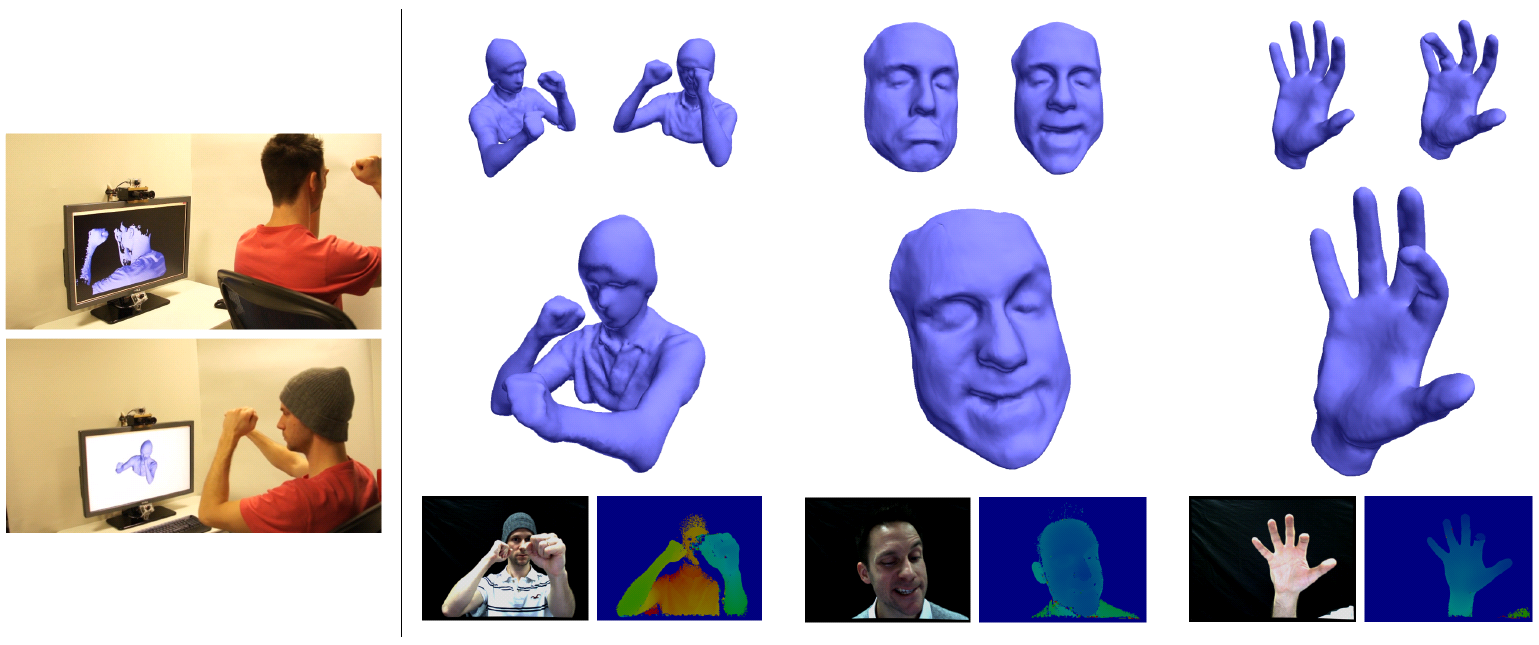
\includegraphics[width=\textwidth]{deformablesTeaser.png}
  \caption{Our system enables the real-time capture of general shapes undergoing non-rigid deformations using a single depth camera.}
  \label{fig:deformables}  
\end{figure}

\paragraph{Dynamic scenes} Capturing 3D environments is no simple feat --- modern 3D reconstruction systems require considerable amounts of memory and computation and are prone to problems such as tracking failure and over smoothing. Alongside work in understanding these environments, I work to augment the technology to capture them, as I believe that real-time capture and reconstruction systems will open up exciting new robotics and augmented/virtual reality applications. One specific area I have looked at is performance capture for deforming 3D objects, shown in Figure~\ref{fig:deformables}. Instead of specializing our reconstruction to a pre-rigged and coded object like a human skeleton, our system minimizes in real time an as-rigid-as-possible deformation energy enabling the capture of arbitrary shapes undergoing non-rigid deformation~\cite{deformables}.

\vspace{0.5cm}
%\begin{flushright}
%Sundar Iyer
%\end{flushright}

\end{small}
%\newpage

%\begin{thebibliography}{deSolaPITH}
% Change font size?
% \tiny, \footnotesize, \small,\normalsize, \large, \Large, \LARGE, and \huge 
%\begin{small}
\begin{footnotesize}

\begin{thebibliography}{}
\bibliographystyle{}

\bibitem[1]{colorByNumbers}
S. Lin, Ritchie D., Fisher M., Hanrahan P., ``Probabilistic Color-by-Numbers: Suggesting Pattern Colorizations
Using Factor Graphs'', {\it SIGGRAPH}, 2013.

\bibitem[2]{exampleSynthesis}
Fisher M., Ritchie D., Savva M., Funkhouser T., Hanrahan P., ``Example-based Synthesis of 3D Object Arrangements'', {\it SIGGRAPH Asia}, 2012.

\bibitem[3]{scenegrok}
Savva M., Chang A., Hanrahan P., Fisher M., Niessner M., ``SceneGrok: Inferring Action Maps in 3D Environments'', {\it SIGGRAPH Asia}, 2014.

\bibitem[4]{actsynth}
Fisher M., Savva M., Li Y., Hanrahan P., Niessner M., ``Activity-centric Scene Synthesis for Functional 3D Scene Modeling'', {\it SIGGRAPH Asia}, 2015.

\bibitem[5]{deformables}
M. Zollhofer, M. Niessner, S. Izadi, C. Rhemann, C. Zach, M. Fisher, C. Wu, A. Fitzgibbon, C. Loop,
C. Theobalt, and M. Stamminger. ``Real-time Non-rigid Reconstruction Using an RBG-D camera''. {\it SIGGRAPH}, 2014.

\end{thebibliography}
\end{footnotesize}

\end{document}

